% !TEX encoding = UTF-8 Unicode

\documentclass[twocolumn,10pt,a4j]{jsarticle}
\usepackage{kougai}

\title{積み上げ型教科の理解を促進させる
教育モデルの提案}
\author{1532009 阿部 希駿  指導教員 須田 宇宙 准教授}
\date{}

\begin{document}

\maketitle

\section{はじめに}

%背景
中学,高校で学習する科目の中で数学と英語は苦手になりやすいと言われている.この2科目の共通点として既に学習した知識を使うことを前提として授業を行う積み上げ型教科という点が挙げられる.積み上げ型教科では単元の内容が複雑になるほど必要な前提知識が多くなり,どの単元の内容が使われているかがわかりにくくなる.そのためその単元の内容を理解をすることが難しくなることが問題点としてあげられる\cite{1}.

%問題点

そこで「単元ごとの繋がりや,その単元を前提知識とする単元の概要をあらかじめ説明することで個々の単元の内容の理解を促進することができる」という仮説を立てた.
本研究では,学生を対象にして実験を行い,この仮説を証明することを目的とする.


\section{積み上げ型教科について}
科目には独立型教科と積み上げ型教科がある.
独立型教科は各単元ごとに完全に別の内容を学習する科目で,国語や社会などがこれに該当する.社会を例とすると「地理」と「公民」の単元には関連性がなく,どちらか一方の内容が理解できていなくても,もう一方の内容を学習するのに支障がない.
これに対して,学習した知識を使うことを前提として授業を行うのが積み上げ型の教科で,数学や英語がこれに該当する.数学を例にすると「正の数・負の数」を前提知識として「文字式」を学習し,「文字式」を前提知識として「方程式」を学習することである.

\section{実験の構想}

本研究では2018年後期に開講される情報数学応用の講義履修者を対象に9週目,10週目,11週目の講義にて対照実験を行う.
図\ref{fig:time}に示すように9週目と10週目に講義を行い,11週目に小テストを行う.

\begin{figure}[H]
\centering
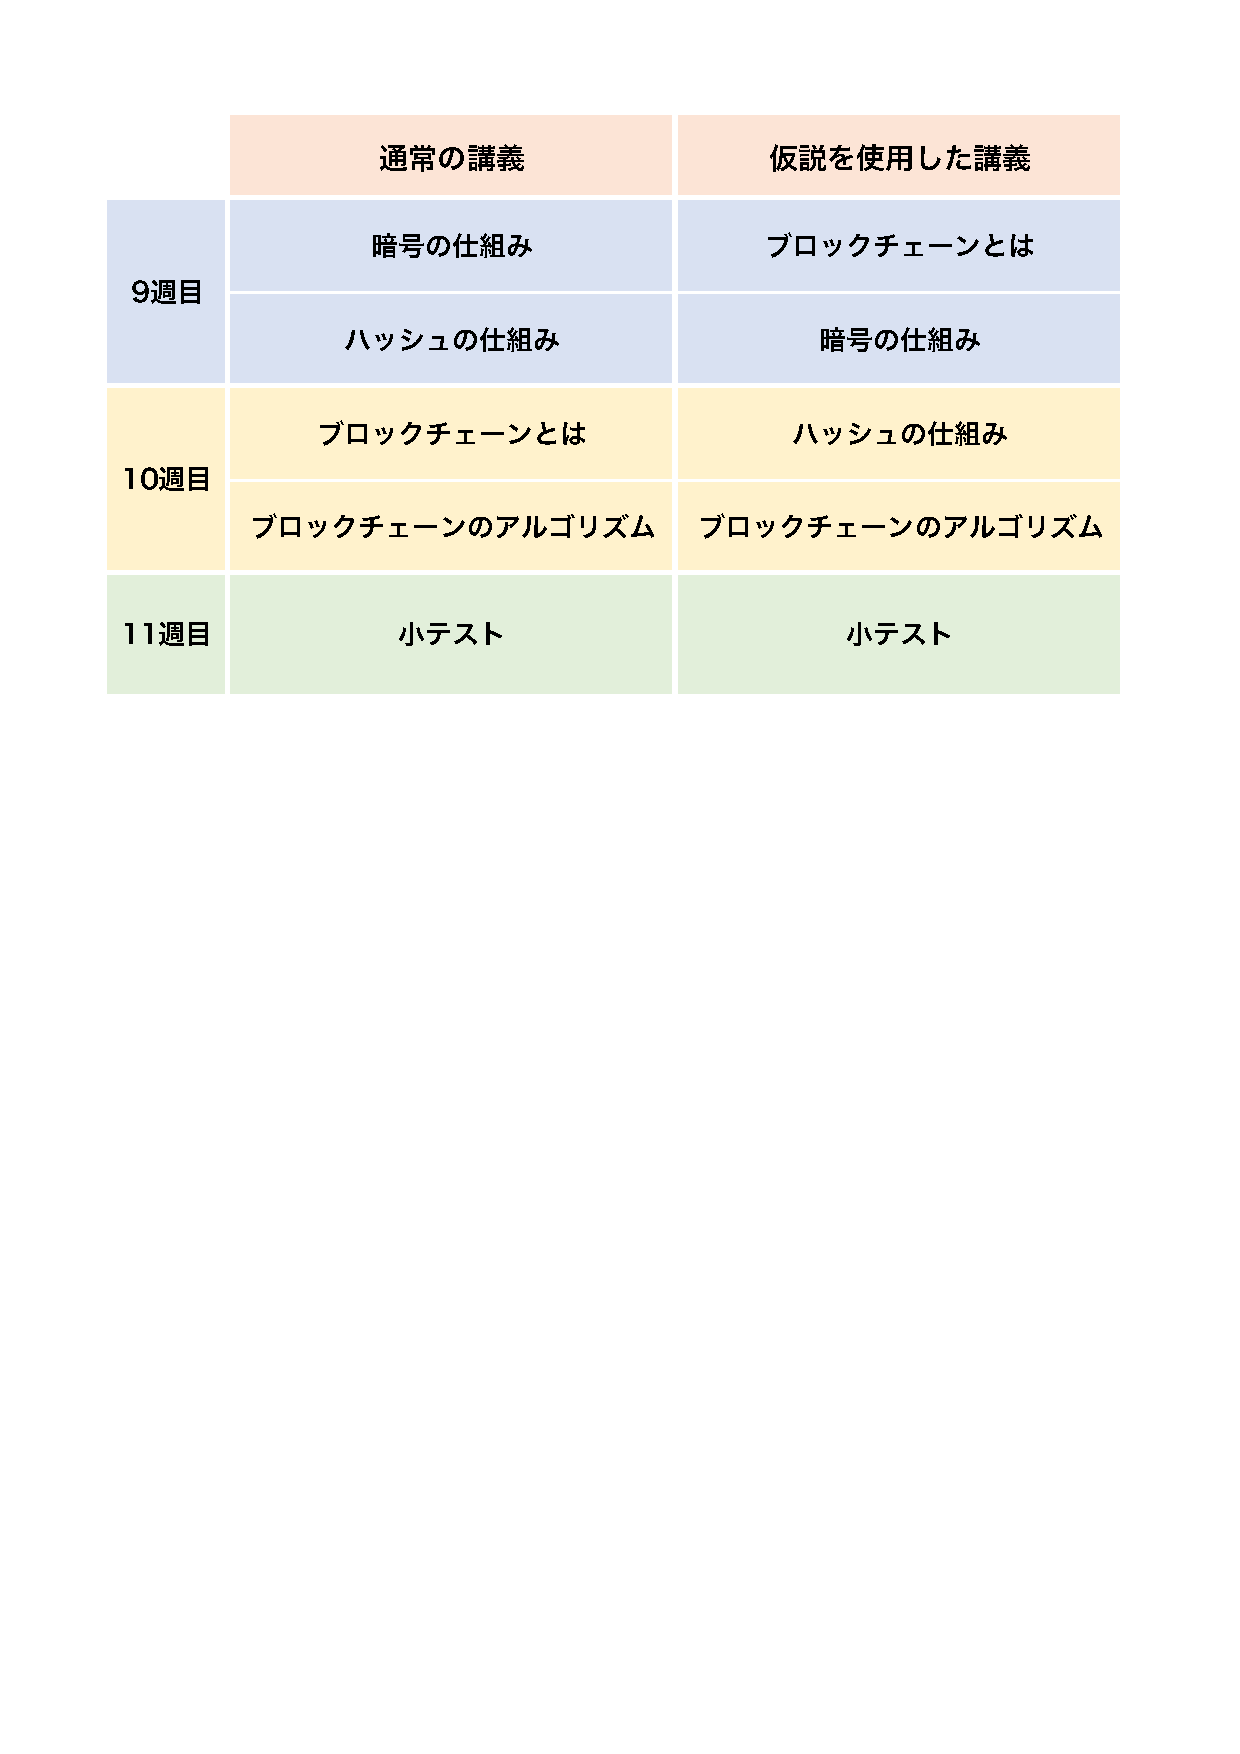
\includegraphics[mediaboxonly=/CropBox,width=9cm]{timeline.pdf}
\caption{実験で行う授業の流れ}
\label{fig:time}
\end{figure}
2限では通常の流れで講義を行い,1限では仮説を基に変更した流れで講義を行う.
仮説を基に変更した講義ではブロックチェーンとはどんなものかを学習した後に暗号とハッシュについて学習し,もう一度ブロックチェーンの学習に戻り詳細に学習する.


小テストでは以下の3項目の問題とアンケートを用意する.
\begin{enumerate}
\renewcommand {\labelenumi}{(\arabic{enumi})}
\item 暗号の仕組み
\item ハッシュと暗号の違い
\item ブロックチェーンの仕組み
\end{enumerate}

アンケートでは講義を受ける以前にブロックチェーンの仕組みについての知識があったかについて尋ねた.
結果の分析は小テストの点数を「暗号・ハッシュ」「ブロックチェーン」の二項目について行う.
また2クラスの中間試験の点数が近いことを元の学力が近いという根拠とする.
そこで小テストの分析対象を中間試験の受験者かつブロックチェーンを講義前に学習していない生徒とした.

小テストの結果,2クラスの点数に差は見られなかった.図\ref{fig:time}では合計点の割合を示す.

\begin{figure}[H]
\centering
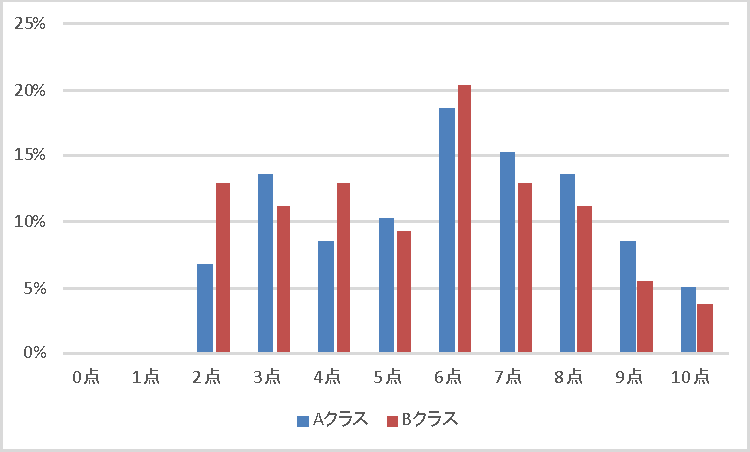
\includegraphics[width=8cm]{total.pdf}
\caption{小テストの合計点の得点割合}
\label{fig:total}
\end{figure}

仮説が証明できなかった原因を3点考えた.
\begin{enumerate}
\renewcommand {\labelenumi}{(\arabic{enumi})}
\item 仮説が間違えている
\item 小テストを行うまでに期間が空いた
\item 実験を行う教科が不適であった
\end{enumerate}



\section{おわりに}
本研究では積み上げ型教科の理解度を上げる仮説を立て,実験を行なった.今回の実験では仮説が正しいと証明することができなかったが,実験の改善点が見つかったため,今後はさらなる実験を行い検証することが望まれる.

\begin{thebibliography}{99}
\bibitem{1}
ベネッセ教育情報サイト:“教科学習が不得意と感じている高校生が9割!そのほとんどが英語と数学に偏るのにはある理由が”, \url{https://www.benesse.jp/kyouiku/201603/20160329-3.html}, (参照 2018-8-14)
\end{thebibliography}

\end{document}